\documentclass[a4paper]{article}
\usepackage[14pt]{extsizes} % для того чтобы задать нестандартный 14-ый размер шрифта
\usepackage[margin=0.7in]{geometry}
\usepackage{multirow}
\usepackage {graphicx}
\usepackage[utf8x]{inputenc} % указать кодировку русского текста
\usepackage[russian]{babel} % указать, что язык текста - русский
\usepackage{fancyhdr}
\pagestyle{fancy}
\usepackage{graphicx}
\graphicspath{{pictures/}}
\DeclareGraphicsExtensions{.pdf,.png,.jpg, .jpeg}
\usepackage{tocloft}
\usepackage{wrapfig}
\usepackage{tikz}
\renewcommand{\cftsecleader}{\cftdotfill{\cftdotsep}}
\begin{document} 
 \begin{titlepage}
\begin{center}
\hfill \break
Министерство науки и высшего образования Российской Федерации\\
ФЕДЕРАЛЬНОЕ ГОСУДАРСТВЕННОЕ АВТОНОМНОЕ ОБРАЗОВАТЕЛЬНОЕ\\ 
УЧРЕЖДЕНИЕ ВЫСШЕГО ОБРАЗОВАНИЯ\\ 
«МОСКОВСКИЙ ФИЗИКО-ТЕХНИЧЕСКИЙ ИНСТИТУТ\\ 
(НАЦИОНАЛЬНЫЙ ИССЛЕДОВАТЕЛЬСКИЙ УНИВЕРСИТЕТ)»\\
(МФТИ)\\
\hfill \break
\hfill \break
\hfill \break
\hfill \break
\hfill \break
\hfill \break
\hfill \break
\hfill \break
\hfill \break
\hfill \break
\hfill \break
ЛАБОРАТОРНАЯ РАБОТА 4.4.1\\
\hfill \break
АМПЛИТУДНАЯ ДИФРАКЦИОННАЯ РЕШЕТКА\\
\end{center}
\hfill \break
\hfill \break
\hfill \break
\hfill \break
\hfill \break
\hfill \break
\hfill \break
\hfill \break
\hfill \break
\hfill \break
\begin{tabular}{ccc}
Работу выполнила студентка группы Б01-009 & & М.В.Шлапак \\\\
\end{tabular}
\hfill \break
\hfill \break
\hfill \break
\hfill \break
\hfill \break
\hfill \break
\hfill \break
\hfill \break
\begin{center} Долгопрудный 2022 \end{center}
\end{titlepage}
\small
\fancyhead[L] {Амплитудная дифракционная решетка}
\tableofcontents    
\newpage
\section{Цель работы}
Знакомство с работой и настройкой гониометра Г5, определение спектральных характеристик амплитудной решетки.\\

\textbf{В работе используются:}  гониометр, дифракционная решетка, ртутная лампа.
\section{Теоретическая часть}
	\noindent Основное соотношение приближенной теории дифракционной решётки:
	\begin{equation}
	d\sin \varphi_m = m\lambda.
	\end{equation}
	Угловая дисперсия $D$ характеризует угловое расстояние между близкими спектральными линиями:
	\begin{equation}
	D = \frac{d\varphi}{d\lambda} = \frac{m}{d \cos \varphi}=\frac{m}{\sqrt{d^{2}-m^{2} \lambda^{2}}}.
	\end{equation}
	
\section{Экспериментальная установка}
	При работе с дифракционной решёткой основной задачей является точное измерение углов, при которых наблюдаются главные максимумы для различных длин волн. В нашей работе для измерения углов используется гониометр Г5. Принципиальная схема экспериментальной установки приведена на рис 1.\\
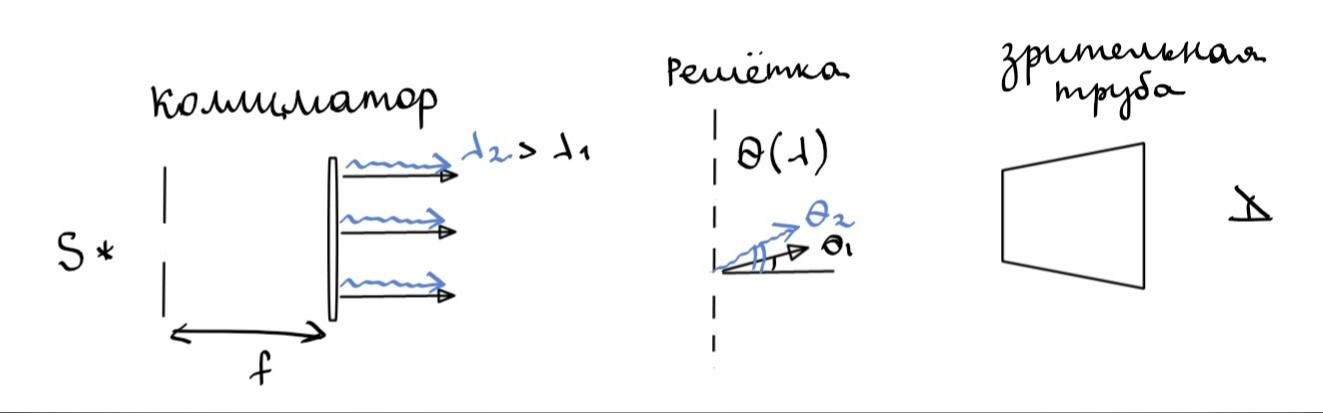
\includegraphics[width=15cm]{inst}\\
\section{Ход работы}
\subsection{ Настройка гониометра}
Провели юстировку гониометра, руководствуясь правилами, изложенными в Приложении. Ознакомились с устройством гониометра и назначением элементов настройки. \\
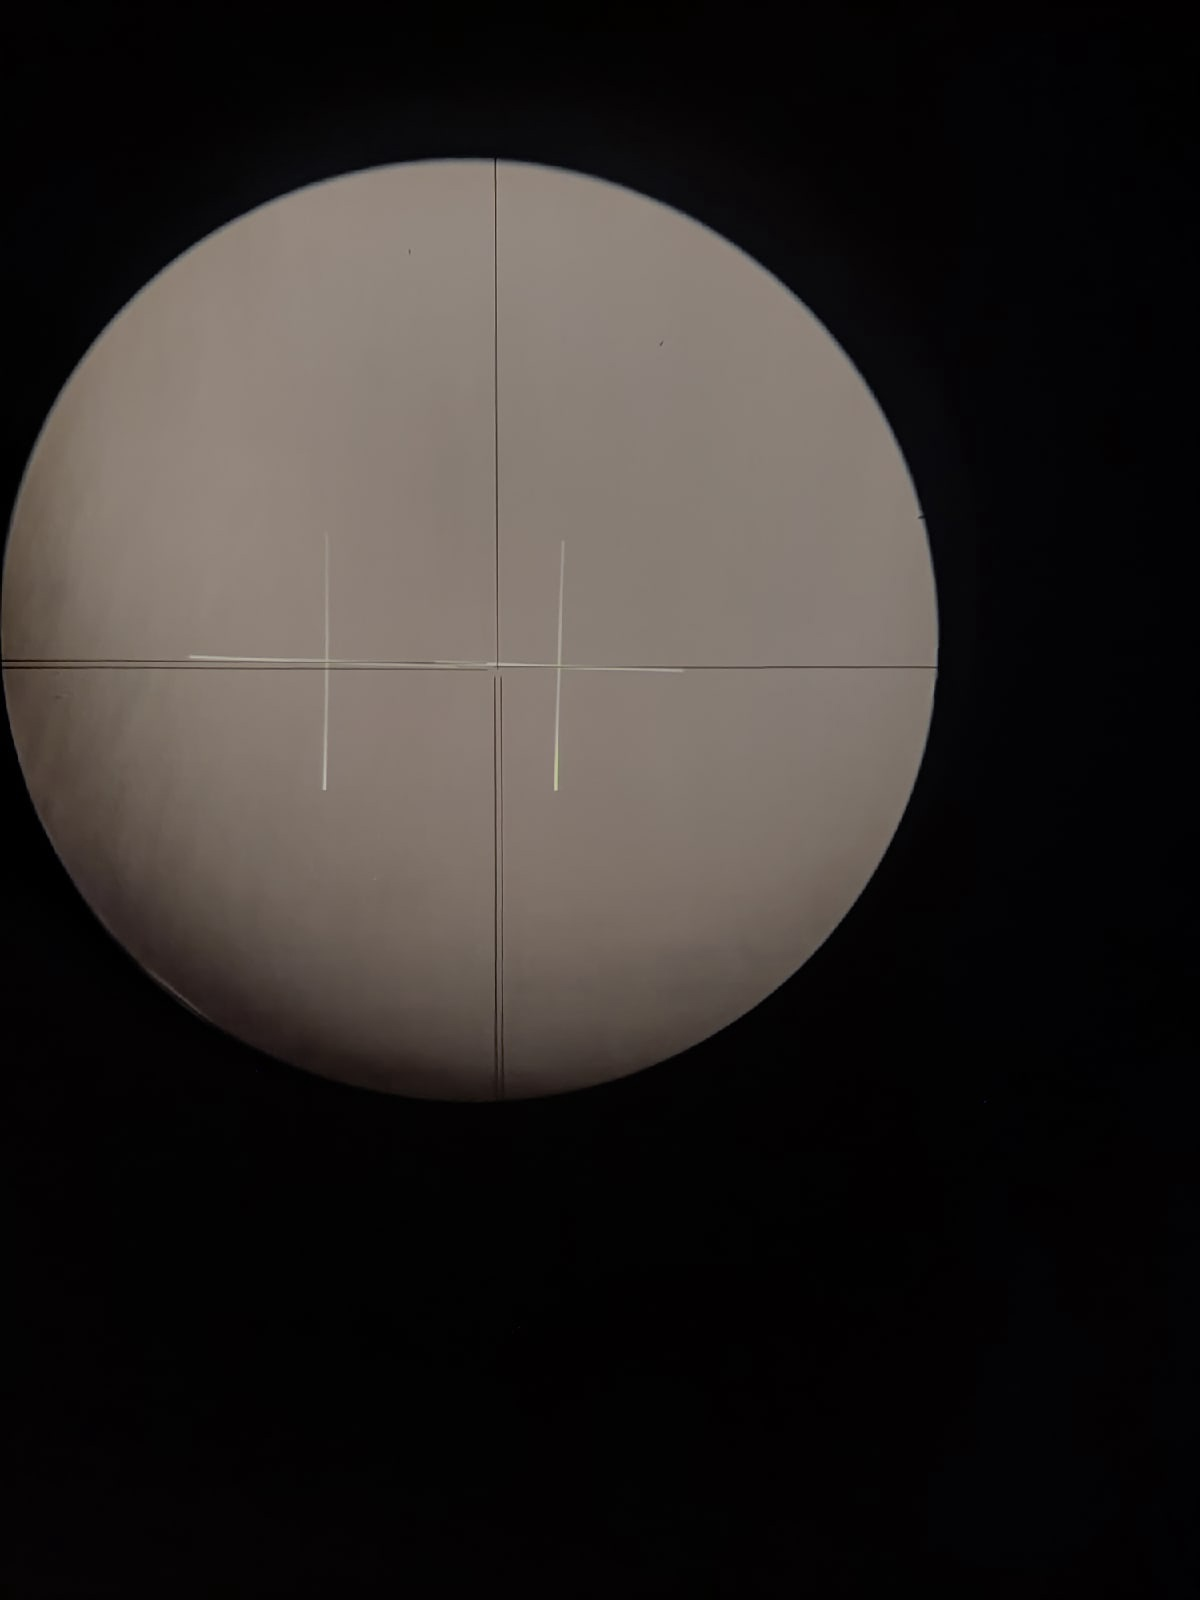
\includegraphics[width=15cm]{p2}\\
\subsection{ Установка решетки}
Установим решетку на столик так, чтобы её плоскость была перпендикулярна оси зрительной трубы и параллельна одному из установочных винтов. В центре поля зрения расположена белая ахроматическая полоса (спектр нулевого порядка). \\
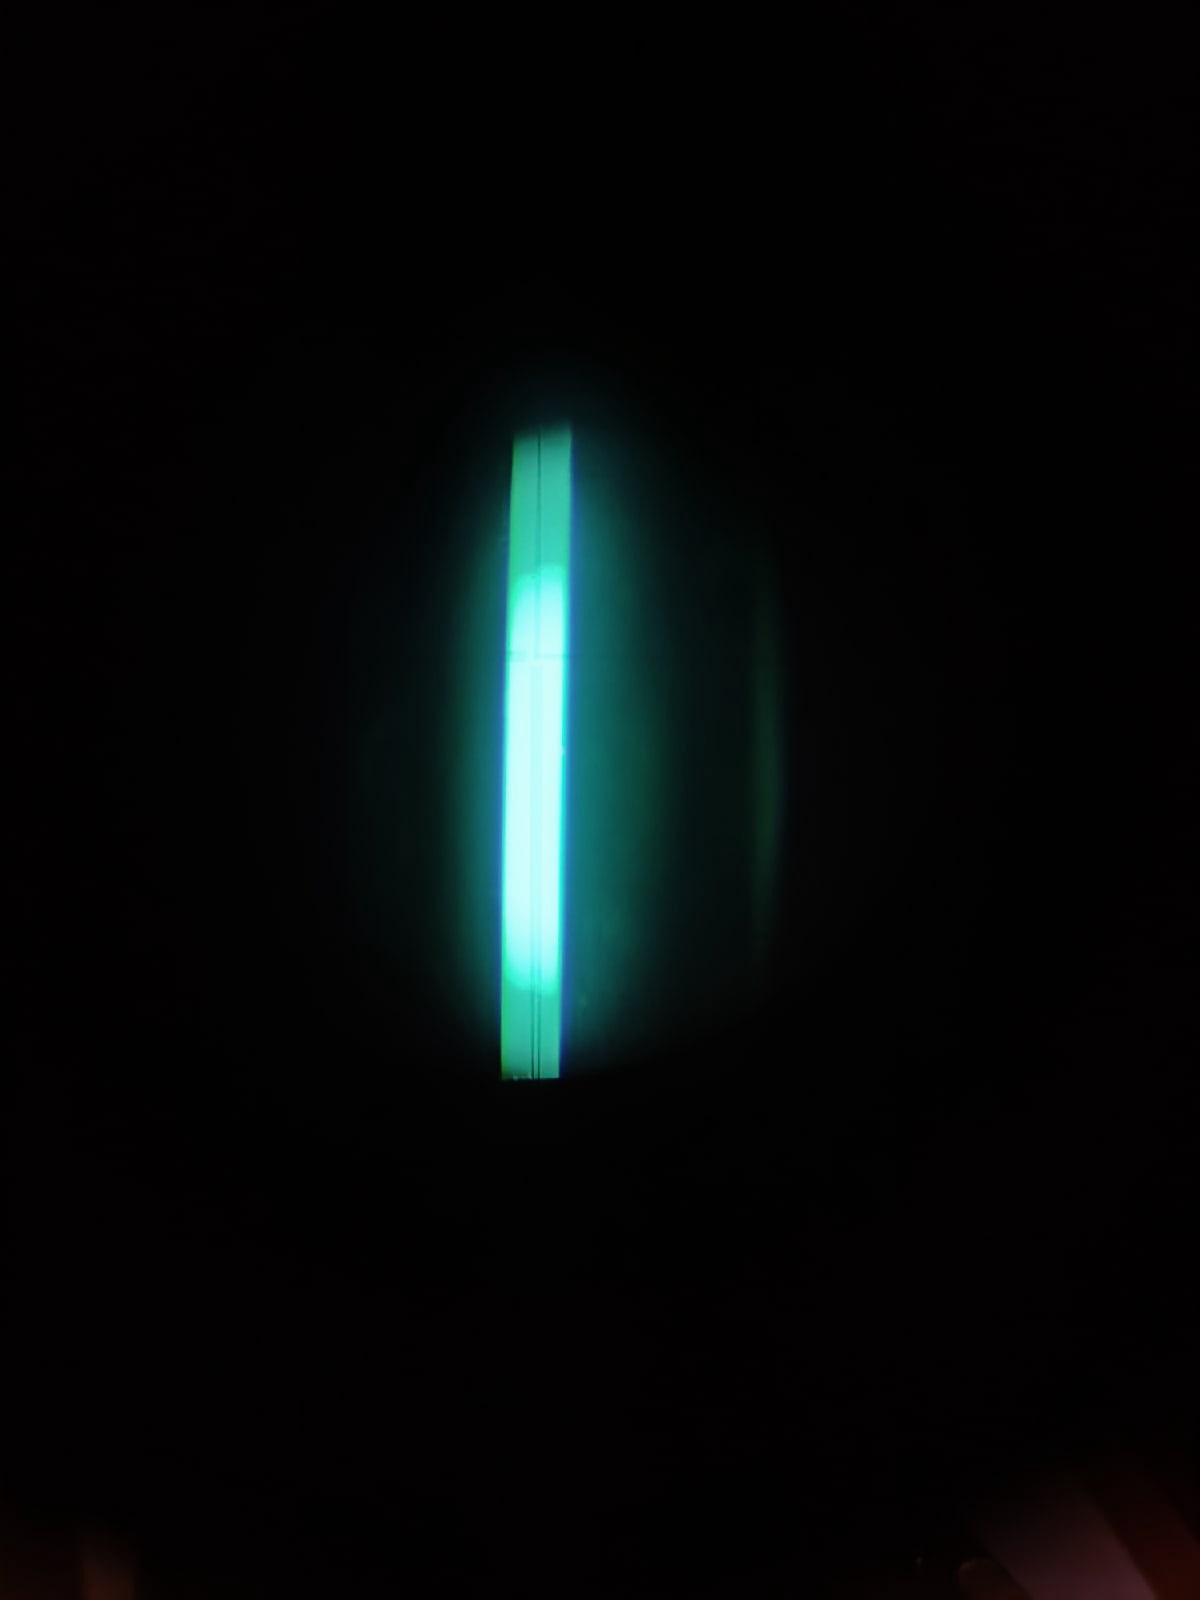
\includegraphics[width=15cm]{p3}\\
\subsection{ Исследование спектра ртутной лампы}
Характеристики решётки: $500$ штр/мм $\Rightarrow$ $d = 0,2 \cdot 10^{-5}$ м.\\
1) Перед выполнением работы убедимся в справедливости формулы $d\sin \phi_m = m\lambda$.\\
Для этого определим углы дифракции для двух ярких линий спектра в одном порядке и убедимся, что $d\sin \phi_m  \sim \lambda$\\
\begin{center}
Угол для первой линии: $163^{\circ}\;4'\;1''$\\
Угол для второй линии: $163^{\circ}\;11'\;37''$\\
\end{center}
Мы брали жёлтые линии, поэтому $\lambda = 578$ нм\\
$$0,2 \cdot 10^{-5} \; \textit{м} \cdot \sin 163^{\circ} \approx 0,58 \; \textit{мкм} \approx 580 \; \textit{нм} \sim \lambda $$ 
Как видно из вычислений, формула верна.\\
\\
2) Измерим с помощью гониометра угловые координаты спектральных линий ртути в $+1$ порядке и построим график зависимости $\sin \phi_{m}$ от длины волны :
\tabcolsep=0.08cm
\begin{center}
\begin{tabular}{|l|l|l|l|l|l|l|l|l|l|}
\hline
велич. & фиол.&син.& гол. & зел. & желт. & желт. & красн. & красн. & $\sigma$\\
\hline
$\phi$&$168^{\circ}11'26''$ & $167^{\circ}12'29''$ & $165^{\circ}23'33''$ & $164^{\circ}05'50''$ & $163^{\circ}11'37''$ & $163^{\circ}4'1''$ & $162^{\circ}06'25''$ & $161^{\circ}26'52''$ & $0,5''$\\
\hline
$\sin \phi$ & 0,205 & 0,221 & 0,252 & 0,274 & 0,289 & 0,291 & 0,307 & 0,318 & 0,0001\\
\hline
$\lambda$, нм & 404,7 & 435,8 & 491,6 & 546,1 & 577,0 & 579,1 & 623,4 & 690,7 & 0,5 \\
\hline
\end{tabular}
\end{center}
Примерное расположение и относительная яркость основных линий взята из методического пособия:\\
\\
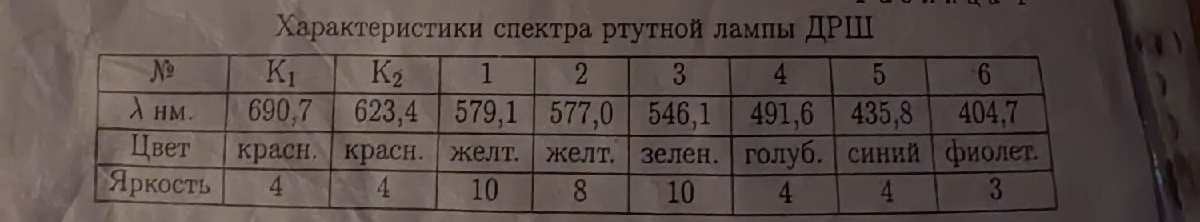
\includegraphics[width=18cm]{p1}\\
Получившаяся зависимость:\\
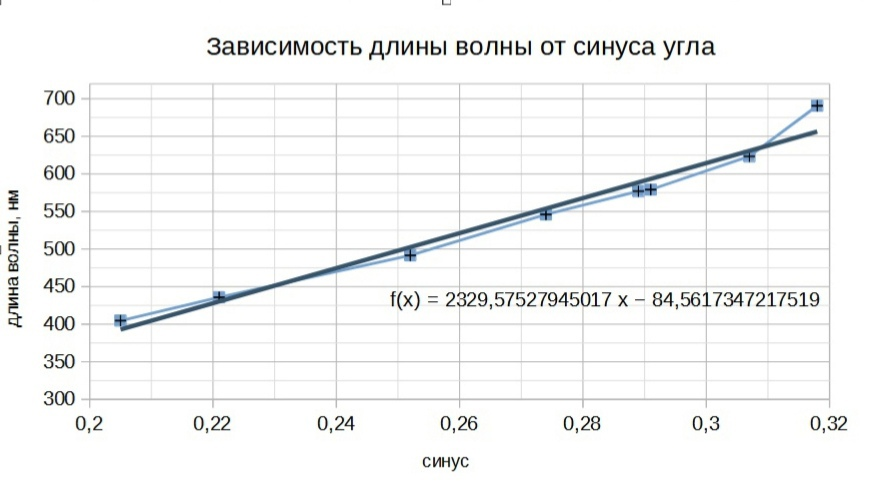
\includegraphics[width=18cm]{g1}\\
По основному соотношению для амплитудной решетки получаем, что период решетки должен выражаться как угловой коэффициент наклона аппроксимирующей прямой:\\
$$d \approx 2329,58\; \textit{нм} \approx 0,233 \cdot 10^{-5}\; \textit{м}$$
Для расчёта погрешности воспользуемся МНК:\\
$$\sigma_d = 893,8 \; \textit{нм} \approx 0,09\cdot 10^{-5} \; \textit{м}$$
Поэтому итоговый ответ для экспериментального значения периода решётки:
$$ d = (0,23 \pm 0,09) \cdot 10^{-5} \; \textit{м}$$ 
2) Для оценки угловой дисперсии решётки измерим угловые координаты линий жёлтого дублета для всех видимых порядков спектра, положительных и отрицательных.\\
Рассчитаем по этим линиям угловую дисперсию в спектрах разного порядка согласно формуле $D = \frac{d\varphi}{d\lambda}$, построим гарфик зависимости угловой дисперсии от порядка спектра, затем сравним эту зависимость с расчётной по формуле  $D = \frac{d\varphi}{d\lambda} = \frac{m}{d \cos \varphi}=\frac{m}{\sqrt{d^{2}-m^{2} \lambda^{2}}}$ для средней длины волны жёлтого дублета $\lambda \approx 578$ нм.\\
\begin{center}
\begin{tabular}{|l|l|l|l|l|}
\hline
длина волны, нм & 577,0 & 579,1\\
\hline
+1 порядок  & $163^{\circ} 11' 37''$ & $163^{\circ} 04' 01''$   \\
\hline
-1 порядок: & $196^{\circ} 24' 21''$ & $196^{\circ} 25' 36''$   \\
\hline
-2 порядок: & $215^{\circ} 05' 22''$ & $215^{\circ} 04' 49''$   \\
\hline
+2 порядок  & $144^{\circ} 20' 39''$ & $144^{\circ} 10' 47''$  \\ 
\hline
\end{tabular}
\end{center}
Тогда угловая дисперсия для спектров разного порядка:\\
\begin{center}
\begin{tabular}{|l|l|l|l|l|l|}
\hline
       порядок      & -2               & -1               & 1                & 2    & $\sigma$        \\
\hline
$d\varphi$, рад & 0,0001584        & 0,00036          & 0,0021888        & 0,0028416   & $1''$    \\
\hline
$d\lambda$, нм  & 2,1              & 2,1              & 2,1              & 2,1    & $0,5$ нм         \\
\hline
$D_{exp}$, рад/м      & $-7,5\cdot10^4$ & $-17,1\cdot10^4$ & $104,2\cdot 10^4$ & $135,3\cdot10^4$& $0,1\cdot10^4$ рад/м\\
\hline
$D_{teor}$, рад/м &$-122,5\cdot10^4$ &$-52,2\cdot10^4$ &$52,2\cdot10^4$ &$122,5\cdot10^4$ &-  \\
\hline
\end{tabular}
\end{center}
Экспериментальная зависимость:\\
\\
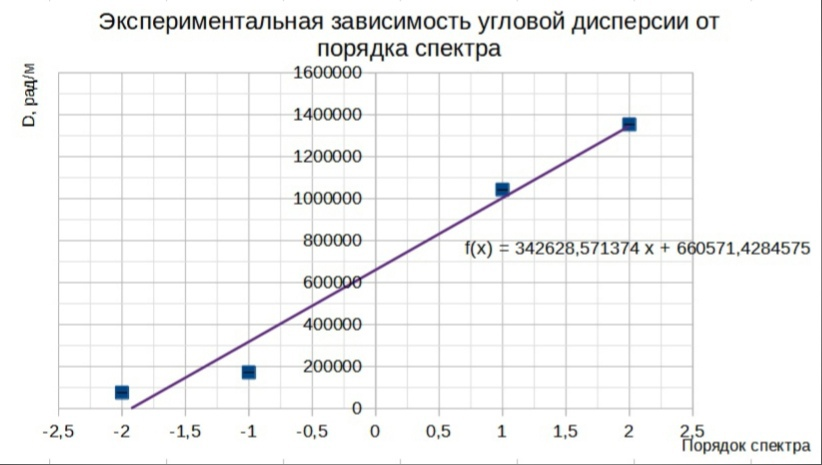
\includegraphics[width=17cm]{g2}\\
Зависимость получается пропорциональной порядку спектра.\\
3) Оценим разрешимый спектральный интервал $\delta \lambda$. Согласно формуле:
$$\triangle \varphi \approx D\delta \lambda = \frac{m}{d\cos \varphi_{m}}\delta \lambda$$
То есть $\delta \lambda \approx \triangle \varphi / D $\\
Тогда разрешимый спектральный интервал: $<\delta \lambda> \approx 7,11$ ангстрем\\
Оценим разрешающую способность для средней длины волны жёлтого дублета по формуле:
$$R = \frac{\lambda}{\delta \lambda}$$
Тогда $R \approx 813$\\
Оценим число эффективно работающих штрихов решётки и её эффективный размер по формуле:
$$N = \frac{R}{m}$$
Тогда $N \approx 407$ (за порядок спектра взят наивысший порядок, то есть 2)\\
\section{Вывод}
В данной работе мы впервые научились применять гониометр для вычисления углов,проверили основное соотношение дифракционной решетки, а также определили некоторые спектральные характеристики нашей амплитудной решётки:\\
\normalsize
\begin{center}
\begin{tabular}{|l|l|l|}
\hline
 $\delta \lambda$ & $R$ & $N$\\
\hline
$7,11$ анг. & $813$ & $407$\\
\hline
\end{tabular}
\end{center}

\end{document}